\documentclass[12pt]{article}
\usepackage[utf8]{inputenc}
\usepackage{hyperref}
\usepackage{listings}
\usepackage{xcolor}
\usepackage{geometry}
\usepackage{graphicx} % For including graphics
\usepackage{minted} % For advanced code listings
\usepackage{enumitem} % For customizing lists
\usepackage{listings-solidity}  % Include Solidity highlighting
\usepackage{amsmath, amssymb, amsfonts} % For mathematical equations

% Define a custom minted style (optional)
\usemintedstyle{colorful} % You can choose from various styles like 'monokai', 'tango', 'colorful', etc.

% Custom color setup
\definecolor{bashtextcolor}{RGB}{0, 0, 0} % Define black color

% Define a new command for inline code using minted
\newcommand{\codeinline}[1]{\mintinline{text}{#1}}

\geometry{a4paper, margin=1in}

\title{Smart Contracts Exercise 09: \\ Vulnerabilities Detection}
\author{}
\date{}

% Define a new command for inline code with a dark background
\newcommand{\codeblack}[1]{%
  \texttt{\colorbox{black!7}{\textcolor{black}{#1}}}%
}

% Define a new command for inline code with a dark background
\newcommand{\codegrey}[1]{%
  \texttt{\colorbox{black!4}{\textcolor{black}{#1}}}%
}

\setitemize{itemsep=5pt, parsep=0pt, label=\small\textbullet} % Set compact spacing and smaller bullets

% Define custom colors (optional)
\definecolor{myURLColor}{RGB}{0, 102, 204} % Example: A shade of blue

\hypersetup{
    colorlinks=true,        % Enable colored links
    linkcolor=blue,         % Color for internal links (e.g., \ref, \cite)
    citecolor=blue,         % Color for citations
    filecolor=magenta,      % Color for file links
    urlcolor=myURLColor     % Color for external URLs
}

% Define a style for code listings
\lstdefinestyle{mystyle}{
    backgroundcolor=\color{lightgray!20},   
    commentstyle=\color{green!50!black},
    keywordstyle=\color{blue},
    numberstyle=\tiny\color{gray},
    stringstyle=\color{red},
    basicstyle=\ttfamily\footnotesize,
    breakatwhitespace=false,         
    breaklines=true,                 
    captionpos=b,                    
    keepspaces=true,                 
    numbers=left,                    
    numbersep=5pt,                  
    showspaces=false,                
    showstringspaces=false,
    showtabs=false,                  
    tabsize=2
}

\lstset{style=mystyle}
% Adding package for header and footer
\usepackage{fancyhdr}
\pagestyle{fancy}

% Define header and footer
\fancyhf{} % Clear current settings
\fancyhead[L]{Smart Contracts Exercise 09} % Left header
\fancyhead[R]{\thepage} % Right header with page number

\renewcommand{\headrulewidth}{0.4pt} % Line below header
% \renewcommand{\footrulewidth}{0.4pt} % Line above footer

\begin{document}

\maketitle
\section{Introduction}

This exercise focuses on general vulnerability detection in smart contracts. We
will explore static code analysis tool Slither to identify vulnerabilities
in contracts from previous exercises. The exercise will also cover the
implementation of unit tests, stateless fuzzing tests, and stateful fuzzing
tests with invariants. We will introduce the Foundry development environment
(this will be new only for students who previously used Hardhat). The primary task involves
writing tests for a simple toy smart contract and then applying this knowledge
to develop more complex tests for the DEX contract from earlier exercise.

\subsection*{Project Setup}

You have two options for working with this exercise: using a Docker container
or local installation. Choose the option that best fits your preferences. For
students who are accustomed to working in the Hardhat environment and using
Docker, it's important to note that this exercise uses a different Docker
image.

\subsection{Using Docker with VS Code}

This option uses Docker to create a development environment with all the
necessary tools and dependencies pre-installed.

\subsubsection*{Prerequisites:}

\begin{itemize}
    \item \textbf{\href{https://www.docker.com/products/docker-desktop}{Docker}} - A platform for developing, shipping, and running applications in containers.
    \item \textbf{\href{https://code.visualstudio.com/}{Visual Studio Code}} - A lightweight but powerful source code editor.
    \item \textbf{\href{https://marketplace.visualstudio.com/items?itemName=ms-vscode-remote.remote-containers}{Dev Containers}} - An extension to VS Code that lets you use a Docker container as a full-featured development environment.
\end{itemize}

\subsubsection*{Setting Up the Project:}

\begin{enumerate}
    \item Visit the following
          \href{https://gitlab.fel.cvut.cz/radovluk/smart-contracts-exercises/-/tree/main/09-Vulnerabilities-Detection/task/task-code}{GitLab
              repository} and clone it to your local machine.
    \item Open the repository folder in VS Code.
    \item When prompted, click ``Reopen in Container'' or use the command palette (F1) and
          run \codegrey{Dev Containers: Reopen in Container}.
\end{enumerate}

\subsection{Local Setup}

If you prefer working directly on your machine without Docker, you can set up
the development environment locally. Before setting up Foundry, ensure that you
have the following installed on your system:

\subsubsection*{Prerequisites}
\begin{itemize}
    \item \textbf{Rust Toolchain} -- Since Foundry is built in Rust, you'll need the Rust compiler and Cargo, Rust's package manager. The easiest way to install both is by using \href{https://rustup.rs/}{rustup.rs}.
    \item \textbf{Bun} -- JavaScript runtime \& toolkit for installing dependencies and running scripts. Install it from \href{https://bun.sh/}{bun.sh}.
\end{itemize}

\noindent
If you don't have Rust installed, you can install it using:

\begin{minted}[bgcolor=gray!5, fontsize=\footnotesize]{bash}
$ curl --proto '=https' --tlsv1.2 -sSf https://sh.rustup.rs | sh
\end{minted}

\noindent
To install Bun, use the following command:
\begin{minted}[bgcolor=gray!5, fontsize=\footnotesize]{bash}
$ curl -fsSL https://bun.sh/install | bash
\end{minted}

\noindent
Open your terminal and run the following command to verify the Rust and Bun installation:

\begin{minted}[bgcolor=gray!5, fontsize=\footnotesize]{bash}
$ rustc --version
$ cargo --version
$ bun --version
\end{minted}

\subsubsection*{Installing Foundry}
You can install Foundry using Foundryup, the official installer:

\begin{minted}[bgcolor=gray!5, fontsize=\footnotesize]{bash}
$ curl -L https://foundry.paradigm.xyz | bash
$ foundryup
\end{minted}

\noindent
This will install the Foundry toolkit, including:
\begin{itemize}
    \item \textbf{Forge} --- Testing framework for Ethereum
    \item \textbf{Cast} --- Command-line tool for interacting with smart contracts
    \item \textbf{Anvil} --- Local Ethereum node for development
    \item \textbf{Chisel} --- Solidity REPL
\end{itemize}

\noindent
Verify the installation by running:

\begin{minted}[bgcolor=gray!5, fontsize=\footnotesize]{bash}
$ forge --version
$ cast --version
$ anvil --version
\end{minted}

\subsubsection*{Setting Up the Project:}

\begin{enumerate}
    \item Visit the following
          \href{https://gitlab.fel.cvut.cz/radovluk/smart-contracts-exercises/-/tree/main/09-Vulnerabilities-Detection/task/task-code}{GitLab
              repository} and clone it to your local machine.
    \item Open a terminal and navigate to the project directory.
    \item Install the project dependencies by running \codegrey{bun install}.
\end{enumerate}

\section{Static Analysis}

Static analysis is a method of examining code without executing it. Unlike
dynamic analysis which examines code during execution, static analysis looks
at the source code or bytecode to find patterns that match known vulnerability
types. If you're using a local setup, you'll need to install Slither first,
while those using the Docker container already have these tools available in
the container.

\subsection*{Slither}

\href{https://github.com/crytic/slither}{Slither} is a static analysis framework that runs a suite of vulnerability detectors, prints visual information about contract details, and provides an API to easily write custom analyses.

\medskip
\noindent
To install Slither using pip3:

\noindent \begin{minipage}{\textwidth}
    \begin{minted}[bgcolor=gray!5, fontsize=\footnotesize]{bash}
$ pip3 install slither-analyzer
\end{minted}
\end{minipage}

\medskip
\noindent
To run Slither on a Solidity file:

\begin{minted}[bgcolor=gray!5, fontsize=\footnotesize]{bash}
$ slither <contract_file.sol>
\end{minted}

\noindent
Now let's try using Slither to identify some vulnerabilities from our exercises. First, we'll analyze the \texttt{src/CatCharity} contract from Exercise 04 -- Re-Entrancy. Run:

\begin{minted}[bgcolor=gray!5, fontsize=\footnotesize]{bash}
$ slither src/CatCharity.sol
\end{minted}

\noindent
Expected output:
\begin{minted}[bgcolor=gray!5, fontsize=\footnotesize]{bash}
INFO:Detectors:
Reentrancy in CatCharity.claimRefund() (src/CatCharity.sol#98-114):
        External calls:
        - (success,None) = address(msg.sender).call{value: donated}() 
        (src/CatCharity.sol#107)
        State variables written after the call(s):
        - donations[msg.sender] = 0 (src/CatCharity.sol#112)
        CatCharity.donations (src/CatCharity.sol#24) can be used in 
        cross function reentrancies:
        - CatCharity.claimRefund() (src/CatCharity.sol#98-114)
        - CatCharity.donate() (src/CatCharity.sol#78-80)
        - CatCharity.donations (src/CatCharity.sol#24)
\end{minted}

As you can see, Slither successfully identified a re-entrancy vulnerability in
the \texttt{CatCharity} contract. It also provided a
\href{https://github.com/crytic/slither/wiki/Detector-Documentation#reentrancy-vulnerabilities}{link}
to documentation about this vulnerability type.

\subsection*{Task 1: Analyze Contracts with Slither}
Analyze all other contracts in the \texttt{src} directory using Slither
(\texttt{SimpleDEX}, \texttt{USDCToken}, \texttt{PiggyBank}) and review
Slither's output. Determine whether the identified issues are actual problems
or false positives. Examine the linked documentation for each reported
vulnerability.

% \subsection*{Mythril}

% \href{https://github.com/ConsenSys/mythril}{Mythril} is an open-source security analysis tool for Ethereum smart contracts. It uses symbolic execution, SMT solving, and taint analysis to detect a variety of security vulnerabilities.

% \medskip
% \noindent
% To install Mythril using pip3:

% \noindent
% \noindent \begin{minipage}{\textwidth}
% \begin{minted}[bgcolor=gray!5, fontsize=\footnotesize]{bash}
% $ pip3 install mythril
% \end{minted}
% \end{minipage}

% \medskip
% \noindent
% To run Mythril on a Solidity file:

% \noindent \begin{minipage}{\textwidth}
% \begin{minted}[bgcolor=gray!5, fontsize=\footnotesize]{bash}
% $ myth analyze <contract_file.sol>
% \end{minted}
% \end{minipage}

\section{Testing in Foundry}

\href{https://github.com/foundry-rs/foundry}{Foundry} provides powerful tools for testing smart contracts, with a focus on flexibility and efficiency. Unlike Hardhat (which uses JavaScript), Foundry uses Solidity for writing tests and scripts. We won't cover all Foundry functions in detail here, but will focus primarily on writing tests. For more information about working with Foundry, visit the project documentation \href{https://book.getfoundry.sh/}{Foundry Book}. Let's now introduce the concept of smart contract testing with a simple example that you'll work with in this exercise. The PiggyBank contract is a simple savings contract where anyone can deposit ETH, but only the owner can withdraw:

\noindent \begin{minipage}{\textwidth}
    \begin{lstlisting}[language=Solidity]
// SPDX-License-Identifier: MIT
pragma solidity =0.8.28;

contract PiggyBank {
    address public immutable owner;
    uint256 public totalDeposits;
    uint256 public totalWithdrawals;
    
    error NotOwner();
    error InsufficientFunds();
    
    constructor() {
        owner = msg.sender;
    }
    
    function deposit() public payable {
        totalDeposits += msg.value;
    }
  
    function withdraw(uint256 amount) public {
        if (msg.sender != owner) revert NotOwner();
        if (amount > address(this).balance) revert InsufficientFunds();
        totalWithdrawals += amount;
        payable(owner).transfer(amount);
    }
}
\end{lstlisting}
\end{minipage}

\medskip
\noindent
\href{https://remix.ethereum.org/?#activate=solidity&url=https://github.com/radovluk/unbreakable-vault/contracts/PiggyBank.sol&lang=en&optimize=false&runs=200&evmVersion=null&version=soljson-v0.8.28+commit.7893614a.js}{PiggyBank in Remix IDE}

\subsection{Unit Testing}

Unit tests verify that individual functions or components of your contract work
as expected in isolation. Documentation on how to write basic tests in Foundry
is available \href{https://book.getfoundry.sh/forge/writing-tests}{here}. Let's
look at an example using our PiggyBank contract. We want to test whether after
calling the \codegrey{deposit()} function, the value of
\codegrey{totalDeposits} will match our deposit.

\noindent \begin{minipage}{\textwidth}
    \begin{lstlisting}[language=Solidity]
function test_Deposit() public {
    uint256 depositAmount = 1 ether;
    
    // Alice makes a deposit
    vm.prank(alice);
    piggyBank.deposit{value: depositAmount}();
    
    // Check totalDeposits
    assertEq(
        piggyBank.totalDeposits(),
        depositAmount,
        "totalDeposits should match deposit amount"
    );
}
\end{lstlisting}
\end{minipage}

\noindent
Another test could verify that if we try to withdraw more money than was deposited into the contract, we receive the appropriate error -- \texttt{InsufficientFunds}.

\noindent \begin{minipage}{\textwidth}
    \begin{lstlisting}[language=Solidity]
function test_RevertWhen_WithdrawExceedsBalance() public {
   // First make a deposit to the piggy bank
   vm.prank(alice);
   piggyBank.deposit{value: 1 ether}();

   // Owner tries to withdraw more than available (should fail)
   vm.prank(owner);
   vm.expectRevert(PiggyBank.InsufficientFunds.selector);
   piggyBank.withdraw(2 ether);
}
\end{lstlisting}
\end{minipage}

\begin{figure}[h!]
    \centering
    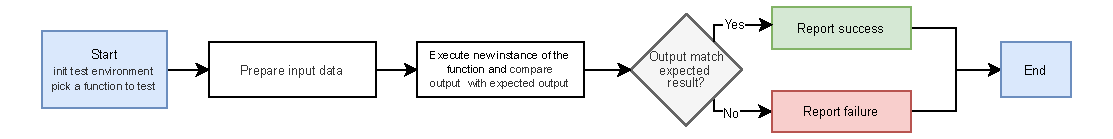
\includegraphics[width=1\textwidth]{unit-testing.pdf}
    \caption{Unit Testing Flow}\label{fig:unit-testing}
\end{figure}

\subsection*{Task 2: Write Unit Tests for PiggyBank}

In the file \texttt{test/PiggyBankUnitTest.t.sol}, complete the missing unit
tests for the PiggyBank contract. Find the functions marked with
\codegrey{TODO} comments and implement them according to the instructions in
the code. The file contains four completed unit tests and four unimplemented
ones that you need to complete. Run the tests using the following command:

\noindent \begin{minipage}{\textwidth}
    \begin{minted}[bgcolor=gray!5, fontsize=\footnotesize]{bash}
$ forge test --match-path test/PiggyBankUnitTest.t.sol -v
\end{minted}
\end{minipage}

\noindent
You can use different verbosity levels to make debugging easier:

\noindent \begin{minipage}{\textwidth}
    \begin{minted}[bgcolor=gray!5, fontsize=\footnotesize]{bash}
-v
    Pass multiple times to increase the verbosity (e.g. -v, -vv, -vvv).
    Verbosity levels:
    - 2: Print logs for all tests
    - 3: Print execution traces for failing tests
    - 4: Print execution traces for all tests, and setup traces for failing tests
    - 5: Print execution and setup traces for all tests
\end{minted}
\end{minipage}

\subsection{Stateless Fuzz Tests}
Fuzzing involves generating random inputs to test your contract's behavior
under various conditions. Unlike unit tests where you provide specific inputs
manually, fuzzing tests automatically generate random (pseudo-random) inputs.
The key advantage is that you can run the same test multiple times with
different input data each time. You can generate completely random input data
or constrain it to specific value ranges. When you run a fuzzing test, it
executes many times in succession, each with different input data, allowing you
to discover edge cases you might not have anticipated. Information about fuzz
testing in Foundry is available here:
\href{https://book.getfoundry.sh/forge/fuzz-testing}{Fuzz Testing}.

\noindent \begin{minipage}{\textwidth}
    \begin{lstlisting}[language=Solidity]
function testFuzz_Deposit(uint96 amount) public {
    // Bound the random input amount to a reasonable range
    uint256 depositAmount = bound(uint256(amount), 0 ether, 99 ether);
    
    // Alice makes a deposit
    vm.prank(alice);
    piggyBank.deposit{value: depositAmount}();
    
    // Check totalDeposits
    assertEq(
        piggyBank.totalDeposits(),
        depositAmount,
        "totalDeposits should match deposit amount"
    );
}
\end{lstlisting}
\end{minipage}

\noindent
Note: In the literature, you'll often encounter confusion between different terms. To be precise, the method described above is called stateless fuzz testing. While we run the function multiple times with different inputs, each run uses a fresh contract instance.

\begin{figure}[h!]
    \centering
    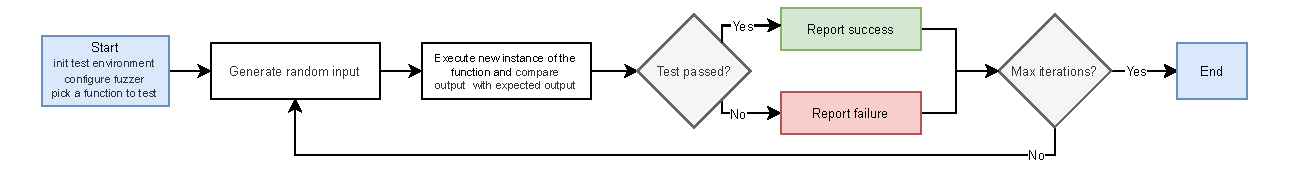
\includegraphics[width=1\textwidth]{fuzz-testing.pdf}
    \caption{Stateless Fuzz Testing Flow}\label{fig:fuzz-testing}
\end{figure}

\subsection*{Task 3: Write Stateless Fuzz Tests for PiggyBank}

In the file \texttt{test/PiggyBankStatelessFuzzTest.t.sol}, complete the
missing fuzz tests for the PiggyBank contract. Find the functions marked with
\codegrey{TODO} comments and implement them according to the instructions in
the code. The file contains four completed fuzz tests and four unimplemented
ones that you need to complete. Run the tests using the following command:

\noindent \begin{minipage}{\textwidth}
    \begin{minted}[bgcolor=gray!5, fontsize=\footnotesize]{bash}
$ forge test --match-path test/PiggyBankStatelessFuzzTest.t.sol -v
\end{minted}
\end{minipage}

\noindent
\textbf{Note:} Test configuration is set in the \texttt{foundry.toml} file. The default setting for stateless fuzz testing is 1000 iterations per test

\subsection{Invariant Testing}

Invariant testing checks that certain properties (invariants) of your contract
remain true regardless of the sequence of operations performed. An invariant is
a specific condition that must always be satisfied no matter which functions
were called on our program, in any order. For example, an invariant for our
PiggyBank contract could be that the current balance of the contract must equal
the difference between all deposits and all withdrawals. This property should
always hold in the system, regardless of how many times the \texttt{deposit()}
and \texttt{withdraw()} functions were called, in what order, and by which
addresses. Properly defining invariants is fundamental to this process. After
defining the invariants, we can simulate the system's execution using stateful
fuzz tests, where different functions will be called in various orders with
different input data, and we'll verify that the invariant is always satisfied.

\noindent \begin{minipage}{\textwidth}
    \begin{lstlisting}[language=Solidity]
/**
* @notice Invariant #1: Contract balance should always equal totalDeposits - totalWithdrawals
* @dev This verifies the core accounting of the contract is correct
*/
function invariant_balanceMatchesAccountingDiff() public view {
    assertEq(
        address(piggyBank).balance,
        piggyBank.totalDeposits() - piggyBank.totalWithdrawals(),
        "Contract balance should equal totalDeposits - totalWithdrawals"
    );
}
\end{lstlisting}
\end{minipage}

\begin{figure}[h!]
    \centering
    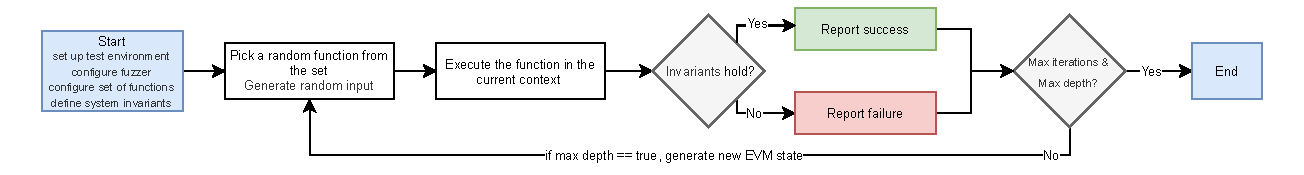
\includegraphics[width=1\textwidth]{invariant-testing.pdf}
    \caption{Invariant Testing Flow}\label{fig:invariant-testing}
\end{figure}

\subsection*{Task 4: Write Invariants for PiggyBank}

In the file \texttt{test/PiggyBankInvariantTest.t.sol}, complete the invariant
definitions for the PiggyBank contract. First, carefully review the
\href{https://book.getfoundry.sh/forge/invariant-testing}{Foundry
    documentation} on invariant testing. Then examine the structure of the
\texttt{test/PiggyBankInvariantTest.t.sol} file to understand how the test is
constructed. Your task is to define at least two additional invariants that
should always hold true for the PiggyBank contract. Run the tests using the
following command:

\noindent \begin{minipage}{\textwidth}
    \begin{minted}[bgcolor=gray!5, fontsize=\footnotesize]{bash}
$ forge test --match-path test/PiggyBankInvariantTest.t.sol -v
\end{minted}
\end{minipage}

\noindent
\textbf{Warning:} after any code change in invariant tests, you need to run the \texttt{forge clean} command because Foundry caches completed tests and only replicates them otherwise.

\noindent
\textbf{Note:} Test configuration is set in the \texttt{foundry.toml} file. The default setting for invariant testing is 256 iterations per invariant with a maximum depth of 150. Each invariant is tested separately against a fresh EVM state.

\section*{Task 5: Implement SimpleDEX Test Suite}

Testing the PiggyBank contract might not have been particularly exciting or
challenging. In the second part of this exercise, you will test the simpleDEX
contract that you're familiar with from Exercise 06 -- Fool The Oracle. To
complete this exercise, you must write all the missing unit tests, all the
missing fuzz tests, and add meaningful invariants. Implement your solution in
the files \texttt{test/SimpleDEXUnitTest.t.sol},
\texttt{test/SimpleDEXStatelessFuzzTest.t.sol}, and
\texttt{test/SimpleDEXInvariantTest.t.sol}.

\medskip
\noindent
Verify your solution with:

\noindent \begin{minipage}{\textwidth}
    \begin{minted}[bgcolor=gray!5, fontsize=\footnotesize]{bash}
$ forge test --match-path test/SimpleDEXUnitTest.t.sol -v
$ forge test --match-path test/SimpleDEXStatelessFuzzTest.t.sol -v
$ forge test --match-path test/SimpleDEXInvariantTest.t.sol -v
\end{minted}
\end{minipage}

\noindent
\textbf{Note:} Foundry follows a specific naming convention for tests and invariants that must be followed, otherwise the tests won't run:

\begin{itemize}
    \item Test files end with \codegrey{.t.sol}
    \item Test contracts inherit from \codegrey{forge-std/Test.sol}
    \item Test functions start with \codegrey{test\_}
    \item Fuzzing tests start with \codegrey{testFuzz\_}
    \item Invariants start with \codegrey{invariant\_}
\end{itemize}

\subsection*{Additional Resources}
\medskip
\noindent
For more resources on fuzzing and invariant testing, check out these links:
\begin{itemize}
    \item \textbf{Even More Resources:} \href{https://github.com/perimetersec/evm-fuzzing-resources?tab=readme-ov-file#evm-fuzzing-resources}{Updated comprehensive list of fuzzing resources}
    \item \textbf{Hands-on Learning:} \href{https://github.com/crytic/building-secure-contracts/tree/master/program-analysis/echidna/exercises}{Practical exercises on fuzzing}
    \item \textbf{Real-world Examples:} \href{https://github.com/perimetersec/public-fuzzing-campaigns-list}{Published professional fuzzing campaigns}
    \item \textbf{Case Study:} \href{https://mirror.xyz/horsefacts.eth/Jex2YVaO65dda6zEyfM_-DXlXhOWCAoSpOx5PLocYgw}{Invariant Testing WETH With Foundry}
    \item \textbf{Video Tutorial:} \href{https://www.youtube.com/playlist?list=PLciHOL_J7Iwqdja9UH4ZzE8dP1IxtsBXI}{Fuzzing Workshop by Trail of Bits}
\end{itemize}

\section{Beyond The Course: The End?}

This course has equipped you with foundational knowledge in smart contract
security. However, the field of blockchain security is vast and constantly
evolving. Here are resources to continue your journey:

\subsubsection*{Interactive Learning Resources -- Development Focus}

Practical hands-on courses focused on smart contract development.

\begin{itemize}
    \item \textbf{\href{https://cryptozombies.io/}{CryptoZombies}} - Interactive lessons for learning Solidity
    \item \textbf{\href{https://speedrunethereum.com/}{SpeedRunEthereum}} - Hands-on challenges to build Ethereum apps
\end{itemize}

\subsubsection*{Interactive Learning Resources -- Security Focus}

Practical exercises similar to those you solved in this course. Ethernaut offers shorter and simpler challenges in the style of the Vaults from Exercise 04, while Damn Vulnerable DeFi is more complex and focuses on DeFi applications, often using real copies of smart contracts.

\begin{itemize}
    \item \textbf{\href{https://www.damnvulnerabledefi.xyz/}{Damn Vulnerable DeFi}} - Challenges focusing on DeFi vulnerabilities
    \item \textbf{\href{https://ethernaut.openzeppelin.com/}{Ethernaut}} - OpenZeppelin's collection of smart contract security challenges
\end{itemize}

\subsubsection*{University Courses}

\begin{itemize}
    \item \textbf{\href{https://github.com/sebischair/bbse}{TUM: Blockchain-based Systems Engineering}} - Blockchain course at Technical University of Munich
    \item \textbf{\href{https://rdi.berkeley.edu/berkeley-defi/f24}{Berkeley DeFi Course}} - Decentralized Finance course at the University of California, Berkeley
    \item \textbf{\href{https://courses.fit.cvut.cz/NIE-BLO/index.html}{FIT ČVUT: NIE-BLO}} - Blockchain Course at Czech Technical University in Prague
\end{itemize}

\subsubsection*{Cyfrin Courses}

Cyfrin is a smart contract security audit company that has published up-to-date practical courses on their website, accessible for free.

\begin{itemize}
    \item \textbf{\href{https://updraft.cyfrin.io/courses/security}{Security and Auditing Full Course}} - Comprehensive guide to smart contract security
    \item \textbf{\href{https://updraft.cyfrin.io/courses/foundry}{Foundry Fundamentals}} - Master the Foundry development environment
    \item \textbf{\href{https://updraft.cyfrin.io/courses/formal-verification}{Formal Verification}} - Learn to use formal methods to verify smart contracts
    \item \textbf{\href{https://updraft.cyfrin.io/courses/advanced-foundry}{Advanced Foundry}} - Take your Foundry skills to the next level
    \item \textbf{\href{https://solodit.cyfrin.io/}{SoloDIT}} - Cyfrin's searchable database of vulnerabilities found in audits
\end{itemize}

\subsubsection*{Competitive Audit Platforms}

Participating in competitive audits is an excellent way to apply your skills in
real-world scenarios, learn from others, and potentially earn rewards:

\begin{itemize}
    \item \textbf{\href{https://code4rena.com/}{Code4rena}} - Competitive audit platform with regular contests and substantial rewards
    \item \textbf{\href{https://www.sherlock.xyz/}{Sherlock}} - Combines security competitions with protocol coverage
    \item \textbf{\href{https://codehawks.cyfrin.io/}{CodeHawks}} - Newer platform with both private and public audit competitions
    \item \textbf{\href{https://immunefi.com/}{Immunefi}} - The largest bug bounty platform in crypto
\end{itemize}

\subsubsection*{Security Tools and Technical Resources}

\begin{itemize}
    \item \textbf{\href{https://github.com/trailofbits/manticore}{Manticore}} - Symbolic execution tool
    \item \textbf{\href{https://github.com/crytic/echidna}{Echidna}} - Fuzzing tool
    \item \textbf{\href{https://github.com/crytic/medusa}{Medusa}} - Fuzzing tool
\end{itemize}

\subsubsection*{Communities and Networking}

\begin{itemize}
    \item \textbf{\href{https://discord.gg/cyfrin}{Cyfrin}} - Active community focused on smart contract security
    \item \textbf{\href{https://discord.gg/qGpsxSA}{Ethereum Research}} - Technical discussions about Ethereum
\end{itemize}

\noindent
It has been a pleasure guiding you through your first steps in smart contract security. Happy hacking, and best of luck on your smart contract security journey!

\end{document}
